\documentclass[crop=false]{standalone}

\begin{document}
	\section{Expected Result}
	本文實驗假設無人機在固定高度,固定速度下前進,並且給定三個參數,1) 給定無人機初始座標位置,2) 給定終點目標 3)隨機生成多個障礙物後,將障礙物位置當成第二個輸入參數。我們預期在獲得輸入參數後,無人機起飛後會首先調整前進方向,由於本文假設無人機以固定速度前進,只需要持續計算與障礙物的距離,並且與障礙物保持安全距離,以及調整方向在並避開障礙物的同時也保持朝向終點方向前進。 如圖1所示:
    
    \begin{figure}[!ht]	
    	\centering
    	
    	\subfloat[Initial\label{subfig-1:DWA}]{%
    		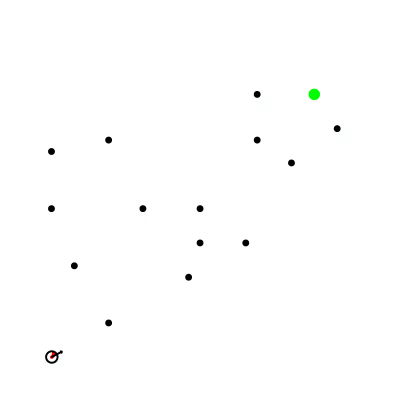
\includegraphics[width=0.2\textwidth]{dwa_frame_0}
    	}
    	\quad
    	
    	\subfloat[Go\label{subfig-2:DWA}]{%
    		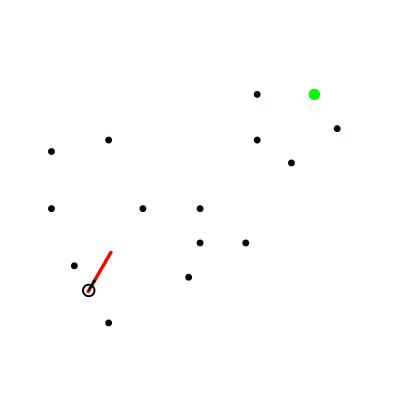
\includegraphics[width=0.2\textwidth]{dwa_frame_1}
    	}
    	\quad
    	
    	\subfloat[Adjusting path to avoid obstacles\label{subfig-3:DWA}]{%
    		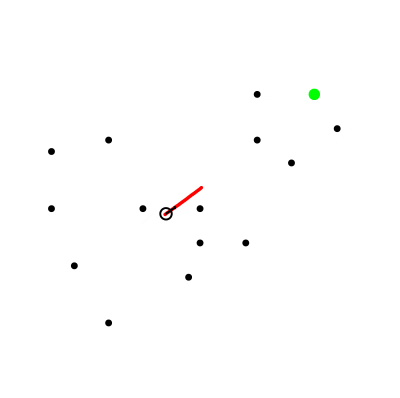
\includegraphics[width=0.2\textwidth]{dwa_frame_2}
    	}
    	\quad
    	
    	\subfloat[Arrived\label{subfig-4:DWA}]{%
    		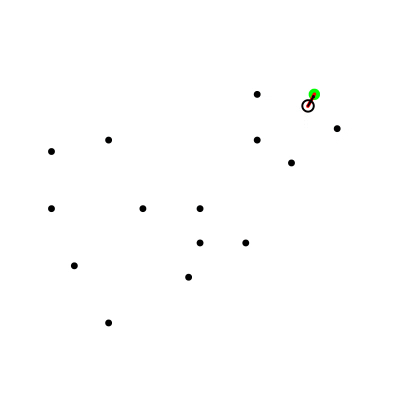
\includegraphics[width=0.2\textwidth]{dwa_frame_3}
    	}

    	
    	\caption{DWA path planning}
    	\label{fig:DWA path planning}
    \end{figure}
\end{document}